\section{Hauptkomponenten der FEM}

Start: Mathematische Formulierung

Ziel: Struktur des Programmcodes mit Einfachheit, Allgemeinheit, Flexibilität und Erweiterbarkeit als Nebenbedingungen (und soll objektorientert sein)

Abstieg von der stetigen in die diskrete Welt \dots
\setcounter{subsection}{0}
\subsubsection{Abstrakte Formulierung}
Hilbertraum $V$, Bilinearform $a: V\times V \to R$, Linearform $f: V \to \R$.
\begin{center}
\framebox{Finde $u \in V$, sodass $a(u, v) = f(v)$ für alle $v \in V = V(\O)$} 
\end{center}
\begin{bemerkung}
  Zur Vereinfachung: 
\item homogene Dirichlet-Randbedingungen
\item kein Petrov-Galerkinverfahren (Ansatzraum $\neq$ Testraum)
\end{bemerkung}
\subsubsection{Diskretisierung A}
\begin{itemize}
\item $V_h \subset V$, $\dim V_h < \infty$, $V_h$ ist der FE-Raum
  \begin{center}
    \framebox{Die numerische Lösung $u_h \in V_h$ soll erfüllen:
$a(u_h, v_h) = f(v_h)$ für alle $v_h \in V_h(\O)$}
  \end{center}
\end{itemize}
\subsubsection{Diskretisierung B}
\begin{itemize}
\item exakte Berechnung von Integralen $a(\cdot, \cdot), f(\cdot)$ nur in Spezialfällen möglich (Quadraturregeln)

$a(\cdot, \cdot) \approx a_h(\cdot, \cdot)$, $ f(\cdot) \approx f_h(\cdot)$, zum Beispiel $\int_E g dx \approx \sum_{i = 1}^{N_Q} g(x_i)w_i$, $w_i \in E$
\end{itemize}
\begin{center}
  \framebox{$u_h \in V_h$: $a_h(u_h, v_h) = f_h(u_h)$ für alle $v_h \in V_h(\O)$} 
\end{center}
\subsubsection{Diskretisierung C}
$V_h(\O) \approx V_h(\O_h)$, $\V_h(\O_h) \not \subset V  = V(\O)$
\subsubsection{Variationelle Formulierung $\to$ LGS}
Definiere Basis $\cB \coloneqq \set{\phi_1, \dots, \phi_N}$ von $V^h$, $N$ ist die Anzahl der Freiheitsgrade (nDoF). Damit für $u_h \in V_h$: 
\begin{align*}
 & v_h = \sum_{j = 1}^N u_j \phi_j\\
 & U = (u_j)_{j = 1}^N \in \R^N \tilde = V_h, u_h \in V_h.
\end{align*}
Für $U \in \R^N$:
\begin{align*}
  \sum_{j = 1}^N u_j a_h(\phi_j, v_h) = f_h, \qquad \forall v_h \in V_h
 \end{align*}
Übung: das ist äquivalent zu: für $U \in \R^N$:
\begin{align*}
  \sum_j u_j \underbrace{a(\phi_j, \phi_i)}_{A_{ij}} = \underbrace{f(\phi_i)}_{F_i}, \qquad i = 1, \dots, N, 
\end{align*}
und mit diesen Abkürzungen können wir kürzer schreiben: für $U \in \R^N$
\begin{align*}
AU = F.
\end{align*}
Damit ist die Methode fast komplett beschrieben. Unbekannt ist noch, welche Basis zu verwenden ist. Die Antwort der FEM lautet, dass sie lokalen Support haben sollte und meist polynomial ist. Die Beschreibung von $\cB$ erfolgt durch ein Gitter/ Mesh $\cT_h$ 
\begin{align*}
  \cT_h = \set{K_i}_{i = 1}^{nE}, \; \inner\left(\bigcup_i K_i \right) = \O_h
\end{align*}
und Konzept der Referenzabbildung $\set{\Phi_K}_{K \in \cT_h}$.

\paragraph{Zusammenfassung:} Wir benötigen 
\begin{itemize}
\item Gitter $\cT_h$ \Lcode{Mesh}
\item Referenzelement $\hat K$ \Lcode{Element}
\item Buchhaltung (lokale ($\hat \phi_i$) bzw. globale ($\phi_i$) Indizierung der Basisfunktionen) \Lcode{DoFManager}
\item FE-Raum $V_h$ (Auswertung in $V_h$) \Lcode{FESpace}
\item Quadraturregeln \Lcode{QuadRule}
\item Operator ($Lu - f = 0$) $\set{a_h, f_h}$ \Lcode{Operator}
\end{itemize}
\paragraph{Programmstruktur}
siehe Skizze (Blatt)
'So einfach wie möglich.'
\paragraph{Flexibilität durch Konzept der Vererbung}
siehe Skizze (Blatt)

Das gilt für alle Klassen.

\subsubsection{Komponenten von Matlab}
Klassendefinition
\begin{verbatim}
classdef Element < handle
properties
...
end 
methods
function Element(obj, name)
obj\_name = name
end
end 
end
\end{verbatim}

Pakete: \Lcode{package}(Ordner), zum Beispiel \Lcode{+meshes}, beinhaltet \Lcode{Mesh.m, Tensormesh.m} \dots, oder \Lcode{+manager}, \Lcode{Work} beinhaltet \Lcode{mesh1} mit \Lcode{elements.txt, nodes.txt}, Daten \Lcode{A.m, f.m} und so weiter. 
\begin{verbatim}
classdef P1 < elements.Element
...
end
\end{verbatim}
Zur Initialisierung: 
\begin{verbatim}
call initPath.m
openInstance('mesh1')
\end{verbatim}
%\datum{04. Dezember 2014}
\subsection{Das Referenzelement}
\begin{itemize}
\item Jedes Element (Kante oder Dreieck, Viereck) des Gitters wund mittels einer Referenzabbildung (Parametrisierung) $\Phi_E$ beschrieben. Der Parameterbereich ist durch das sogenannte Referenzelement gegeben. 
  \begin{enumerate}
  \item Kante: $\hat K_F = [0, 1]$ $\Phi_F: \R \to \R^2: \Phi(\hat K_F) = F$
\item Dreieck: $\hat K_T = \set{(\hat x,\hat y) \in [0, 1]^2: \; 1- \hat y \geq  \hat x}$, $\Phi_T: \R^2 \to \R$
\item Vierecke $\hat K_R = \set{(\hat x, \hat y) \in [0,1]^2}$, $\Phi_R: \R^2 \to \R^2$. 
  \end{enumerate}
\item Für eine wohldefinierte Konstuktion von $V_h$ ist eine Festlegung von
  \begin{itemize}
  \item der Nummerierung der Ecken
  \item der Nummerierung der Kanten
  \item der lokalen Orientierung der Kanten notwendig
  \end{itemize}
  \begin{enumerate}
  \item Kante: eine Kante, linker Endpunkt: 1, rechter Endpunkt: 2
  \item Dreieck: 1: beim rechten Winkel, 2, 3: weiter im positiven Sinn. Kanten: wie Punkte, jeweils rechte Kante
\item Viereck: 1. Punkt links unten, 2. rechts unten, 3. links oben, 4. rechts oben, untere Kante ist die erste, dann im math. pos. Sinn  
  \end{enumerate}
\item Auf $\hat K$ wird durch die Definition von (lokalen) Basisfunktionen $\cB \coloneqq \set{\hat \phi_i}_{i = 1}^{\Lcode{nB}}$ ein beliebiger, endlichdimensionaler Funktionenraum definiert. $(\hat V_h = \Span \cB)$. 
\item Aufgabe des Referenzelementes im Code: 'Auswertung der $\hat \phi_i$s und deren Ableitungen in beliebigen Punkten $\hat x \in \hat K$'. 
\end{itemize}
Das heißt konkret: Die KLasse \Lcode{element.Element} stellt die Methode
\begin{center}
  \Lcode{B = getBasis(obj, points, order)}
\end{center}
bereit, wobei \Lcode{points} $\in \R(nP, nD)$, \Lcode{order} $\in{0, 1, \dots}$,\Lcode{B}$\in \R(nB, nP, [nD, nD])$.
im Element: 
\begin{verbatim}
function B = getBasis(obj, points, order)
switch order
case 0
B = obj. getD0Basis(points)
case 1
B = obj. getD1Basis(points)
    end
end
\end{verbatim}
Die in Element abstrakten Methoden \Lcode{getD\_Basis} müssen in konkreten Elementen definiert werden. (s. Skizze)
\subsubsection{Dreieckselemente}
\begin{enumerate}
\item Lineare $L_1$-Elemente

  \begin{align*}
&    \hat \phi_1 = 1 - \hat x - \hat y\\
&    \hat \phi_2 = \hat x\\
&    \hat \phi_3 = \hat y\\
&    \hat \psi_1 = 1-\hat x\\
&    \hat \psi_2 = \hat x\\
  \end{align*}
\item $P_2$-Elemente

  \begin{align*}
    \hat \phi_i(\hat x _j) = \delta_{ij}
  \end{align*}
Es sind noch Koeffizienten aus diesen Bedingungen ermitteln. 
\item hierarchisches $P_2$-Element
  \begin{align*}
    & \hat \phi_i(\hat x _j) = \delta_{ij}, \quad i, j \in \set{1, 2, 3}\\
    & \hat \phi_i \in P_1, \qquad i = 1, 2, 3\\
    & \hat \phi_{4 - 6} \text{ wie } P_2
  \end{align*}
\item Crouzeix-Raviart Element
  
  \begin{itemize}
  \item linear
  \item Lagrange
  \item Stückpunkte = Kantenmittelpunkte
  \end{itemize}   
  \begin{align*}
    & \hat \phi _1 = 2 \hat x + 2 \hat y - 1\\
    & \hat \phi _2 = 1 - 2 \hat x\\
    & \hat \phi _3 = 1 - 2 \hat y
    \end{align*}
    ($\hat x_i$ Kantenmittelpunkte)
\end{enumerate}
\subsubsection{Viereckselemente}
\begin{enumerate}
\item $Q_1$- Element
  \begin{align*}
    &\hat \phi_1 = (1- \hat x)(1- \hat y)\\
    &\vdots\\
    &\hat \phi_4 = \hat x \hat y
  \end{align*}
$\psi_i$ wie bei $P_1$. 
\item $Q_2S$-Element (Serendipity-Element)
  \begin{align*}
   & \cB = \cB_{Q_1} \cap \set{\hat \phi_i}_{i = 5}^8\\
   & \hat \phi _5 = \hat x (1 - \hat x)(1- \hat y) \\
   & \vdots\\
  \end{align*}
('Quadratische Kantenbubbles')
\end{enumerate}
\begin{bemerkung*}
  Auch parametrische Elemente möglich, welche eine ganze Klasse abdecken, zum Beispiel 'Parameter entspricht Polynomgrad/Raumdimension'
\end{bemerkung*}
Ziel der Übung: 
\begin{itemize}
\item Implementierung möglichst vieler konkreter Elementklassen
\item Routine zur Visualisierung der Basis und Ableitungen 
\end{itemize}
\subsubsection{Finite Elemente beliebiger Ordnung} (zunächst für Vierecke)

Betrachte $Q_1, Q_2, Q_3 \to Q_p$, $p$ Parameter

Basisfunktionen und Ableitungen beliebiger Ordnung werden nicht mehr hart codiert, sondern auf Anfrage bei der Auswertung 'virtuell' generiert (Rekursionsformeln)

\paragraph{Vorgehen:}
\begin{enumerate}
\item 1D-Formfunktionen
  \begin{definition*}
    Eine \markdef{Formfunktion} $N_k : I \coloneqq[-1, 1] \to \R$ ist eine Funktion der Form 
    \begin{align*}
      &N_0(x) \coloneqq \frac 1 2(1 - x)\\
      &N_1(x) \coloneqq \frac 1 2(1 + x)\\
      &N_k(x) \coloneqq   \frac {1}{\nnorm{L_{k-1}}_0} \int_{-1}^1 L_{k-1}(t) dt, \qquad k = 2, 3, \dots
    \end{align*}
mit den Legendrepolynomen $L_k$, $L_k(1) = 1, L_k(-1) = (-1)^k$. Es gilt
\begin{align*}
  N_k(\partial I) = 0, 
\end{align*}
weil 
  \end{definition*}
  \begin{bemerkung*}
    \begin{itemize}
    \item Anpassung der Approximationsgüte besonders leicht (p-Adaption, Serendipity-Element)
    \item  $\set{N_k}_{k = 0}^p$ bilden eine Basis in $\Pi_p(I)$
    \end{itemize}
  \end{bemerkung*}
\item Effiziente Auswertung der $N_k$'s

Ohne Beweis gelten folgende Beziehungen:
  \begin{enumerate}
  \item $L _{k-1} = \frac 1 {2k-1} \frac d {dx}(L_k - L_{k-2})$
  \item $L_k = J_k^{(0, 0)}$, $J_k^{(\alpha, \beta)}$ sind die orthogonalen Polynome bezüglich $(f, g)_* \coloneqq \int_I(f, g)(x)(1- x)^{\alpha}(1+x)^\beta dx$, $\alpha, \beta > -1$. 
\item $\frac {d^n}{dx^n} J_k^{(\alpha, \beta)}(x) =  2^{-n} \frac {\Gamma(k+ n+ \alpha + \beta -1)}{\Gamma(\alpha + \beta + k + 1)} J_{k-n}^{\alpha + n, \beta + n}(x)$
\item Jacobi-Polynome lassen sich schnell, stabil mit Rekursionsformeln berechnen
  \end{enumerate}
\item Redefiniere $N_k \to N_k$
  \begin{align*}
    \nu: &[0, 1] \to [0, 1]\\
    & x \mapsto 2x -1\\
& N_k  \coloneqq N_k \circ \nu: [0, 1] \to \R
  \end{align*}

$\hat K_I \coloneqq[0, 1]$, $\cB_p = \set{\hat \phi_k \coloneqq N_{k-1}| \; k = 1, \dots, p+1}$
 \end{enumerate}
\begin{uebung}
  Zeige: aus (*), (1) und (3) folgt $\frac {d^n}{dx^n} N_k(x)= $ Expr. (Jac. Pol.) 
\end{uebung}
\begin{uebung}
  Implementiere
$y = \text{getJacobi}(x, k, \alpha, \beta)$

$y = \text{getShapeFunctions}(x, k, n)$ mit der Ordnung $k$, $n$.
\end{uebung}
Nun für das Viereckselement $\hat K_R \coloneqq [0, 1]^2$: 

\begin{itemize}
\item Tensorprodunkt $\hat K_R \coloneqq \hat K_I \times \hat K_I$, $\cB_{Q_p} \coloneqq \cB_I \times \cB_I$. %tensor?!

$B_1$: Viereckbezogene Basisfunktionen, $B_1 = \set{\hat \phi_i, i = 1, \dots, 4}$, $\hat \phi_1, (\hat x, \hat y) = N_0(\hat x) N_0 (\hat y)$, $\hat \phi_2$ bis $\hat \phi_4$ analog. 

$B_2$: viermal $(p-1)$ Kantenbubbles
\begin{align*}
  &B_2 = \bigcup_{i = 0}^{p-2} \set{\hat \phi_{4 + 4i+ k} | \; k = 1, \dots, 4}\\
  &\hat \phi_5 \coloneqq N_2(\hat x) N_0(\hat y)
\end{align*}
$\hat \phi_6$ analog. 

$B_3$: $(p-1)^2$ innere Basisfunktionen $B_3 = \set{\hat \phi_{4p + k} | k = 1, \dots, (p-1)^2}$, $\cB_{Q_p} = B_1 \cup B_2 \cup B_3$.
\end{itemize}
%\datum{09. Dezember 2014}

\subsection{Das Gitter}

Hauptaufgabe:
\begin{itemize}
\item Beschreibung /Approximation von $\O$ durch $\O_h$
\item Auswertung der Referenzabbildung $\set{\Phi_E}_E$ (siehe 1.1)
\item Auswertung von Daten in lokalen Punkten
\item Codieren von Konnektivitäts- und Nachbarschaftsbeziehungen 
\end{itemize}
Weitere Aspekte: 
\begin{itemize}
\item Verfeinerung
\item globale Suche (Visualisierung von $V_h$)
\item Visualisierung des Gitters
\end{itemize}
\subsubsection{Datenstrukturen und Konnektivität (2D)}
Hauptstrukturen:
\begin{enumerate}
\item Punktwolke $\cN$ \Lcode{nodes} $\in \R(nN, 2)$ (\Lcode {nN}: number of nodes) (Rohdaten)
\item Elemente $\cE = \set{(n_1, n_2, n_3)| \; n_i \in \N}$ (\Lcode{elem} $\in \N(nE, 3)$) (Rohdaten)
\item Kanten des Gitters $\cF = \set{f_k = (n_1, n_2)| \; n_i \in \N}, \; k = 1, \dots, nF$ (\Lcode{faces} $\in \N(nF, 2)$)
\item Abbildung \Lcode{n2F}$: \cN \times \cN \to \set{0, \dots, nF}$ (\Lcode{sparse(faces, faces(:., [2, 1]), [(1:nF)',(1: nF)])})
\item Abbildung \Lcode{n2E}$: \cN \times \cN \to \set{0, \dots, nE}$
\end{enumerate}
Es sind weitere Datenstrukturen nötig und möglich:
\begin{itemize}
\item benachbarte Elemente einer Kante ($\cF \to \cE \times \cE$)
\item benachbarte Kanten eines Elements ($\cE \to \cF^3$) (Dreiecke)
\item benachbarte Elemente eines Elements
\item benachbarte Kanten eines Knotens $\cN \to \bigcup_{ k > 0} \cF^k$
\end{itemize}
\begin{beispiel} Skizze siehe Blatt

  nodes: 
  \begin{tabular}{c c}
    0.0 & 0.0 \\
    1.0 & 0.0 \\
    1.0 & 1.1 \\
 \dots & \\
    0.0 & -1.0 
  \end{tabular}

elem: 
\begin{tabular}{c c c c}
  1 &2 &4 & 3\\
  8 &7 &1 & 2\\
  7 &6 &2 & 5
\end{tabular}

faces:
\begin{tabular}{c c }
  1 & 2 \\
7 & 8 \\
\dots & \\
5 & 6
\end{tabular}
\end{beispiel}

\subsubsection{Orientierung}
Problem: Die gemeinsame Kante zweier Dreiecke ist in den beiden Elementen entgegengesetzt orientiert.
\begin{itemize}
\item  wichtig bei $C^0$-Elementen: Vertauschung von Knoten
\item verschiedene lokale Koordinatensysteme auf einer Kante möglich (siehe 1.3 DoF-Manager)
\item lokale Speicherung der globalen Orientierung
  \begin{align*}
    \Lcode{orient} = 
    \begin{bmatrix}
      1 & 1 & -1\\
      -1 & 1 &-1 \\
    \end{bmatrix}
  \end{align*}
\end{itemize}
  \begin{bemerkung*}
    Verallgemeinerung auf 3D (Flächen) möglich, allerdings mit mehr als 2 Orientierungen (Tetraeder: 6, Quader: 8)
  \end{bemerkung*}
\subsubsection{Hierarchieinformationen}

Motivation:
\begin{itemize}
\item effiziente Umsetzung von Verfeinerung und Vergröberung
\item Multigrid-solver
\end{itemize}
Vorgehen:
\begin{itemize}
\item Das Gitter speichert seine Geschichte, also den Zustand auf konkreten Levels (level 0 ist das feinste Level (\Lcode{leaf level}))
\item Jedes Element bekommt folgende zusätzliche Informationen:

    \Lcode{level}: $\R^{nE \times 2}$ \dots in welchen Levels ist das jeweilige Element aktiv (leaf)

\Lcode{child}:  $\R^{nE \times 10}$ \dots welche 'Kinder' hat ein (nicht aktives) Element

\Lcode{father}:  $\R^{nE \times 2}$ \dots welches 'Vaterelement' wurde wie verfeinert
\end{itemize}
\begin{beispiel}
  Skizze siehe Blatt


  \begin{tabular}{c c c c c }
    \# & \Lcode{level} & \Lcode{elem}& \Lcode{child} & \Lcode{father}  \\
1 &  0 0 & 2 3 4 & 0 \dots 0 &  0 0\\
2 &  0 0 & 2 4 3 & 0 \dots 0 &  0 0 \\ \hline
1 &  0 1 & 1 3 4 & 0 \dots 0 &  0 0\\
2 &  1 1 & 2 4 3 & 0 0 0 0 0 0 3 4 5 6 &  0 0\\
3 &  0 0 & 1 7 6 & 0 \dots 0 &  2 7\\
4 &  0 0 & \dots & 0 \dots 0 &  2 8\\
5 &  0 0 & \dots & 0 \dots 0 &  2 9\\
6 &  0 0 & \dots & 0 \dots 0 &  2 10
  \end{tabular}
\end{beispiel}
Beliebige Verfeinerungshierarchien können erreicht werden. Eine analoge Hierarchie ist auch für Kanten nötig.

\subsubsection{Referenzabbildung}
Operationen auf physikalischen Elementen (Assemblierung, Integration, Auswertung) werden mittels Referenzabbildung oder auf dem Referenzellemt durchgeführt(pull-back) $\Phi_K: \hat K \to K$ ($C^\infty$-Diffeomorphismus). Beschreibung von $\Phi_K$:
  \begin{enumerate}
  \item $\Phi_K (\hat x) = p_1 +
    \begin{pmatrix}
      p_2 - p_1 & p_3 -p_1
    \end{pmatrix}
\hat x$
\item alternative Beschreibung: 
  \begin{align*}
    \Phi_K (\hat x) = p_1 \hat \phi_1(\hat x) + p_2 \hat \phi_2(\hat x) + p_3 \hat \phi_3(\underline{\hat x}) = \sum_{i = 1}^3 p_i \hat \phi_i(\underline{\hat x})
  \end{align*}
\item Verallgemeinerung auf Elemente höherer Ordnung
  \begin{align*}
    \Phi_K \underline{\hat x} = \sum_{i = 1}^{nB} c_{i, k} \hat \phi_i (\underline{\hat x})
  \end{align*}
  \end{enumerate}
  \begin{bemerkung*}
    Analog wird eine Abbildung für Kanten beschrieben. 
  \end{bemerkung*}

%\datum{11.Dezember 2014}
\subsubsection{Effiziente Auswertung von $\Phi_K$}
Interface \Lcode{R = evalReferenceMap(points, order)}, \Lcode{points}$\in R(nP, nD)$, \Lcode{order}$\in \N$, \Lcode{R}$\in \R(nDim, nE, dP, nO)$
mit nDim: Raumdimension, nE: Elementanzahl, nP: Punktanzahl, nO: Ableitungen mit
\begin{align*}
  points, order \mapsto \set{\sum_{ i = 1}^{nB} c_{i, k}D^n \hat\phi_i(\hat x_{k})}_{k= 1, \dots, nP, k = 1, \dots, nE}
\end{align*}
\begin{enumerate}
\item Berechnung von 
  \begin{align*}
%    \set{\phi_i ( \underbar{ \hat{x}_k}) }_{i, k}
  \end{align*}
\begin{align*}
  B \coloneqq \operatorname{ShapeElem.getBasis}(point, order) \in \R(nB,nP, nO)
\end{align*}
\item Bestimme $\set{c_{i, k}}_{i, k}$ aus dem Knotenvektor (\Lcode{nodes})
  \begin{align*}
    A \coloneqq \operatorname{obj.nodes}(\operatorname{obj.elem}, :) \in \R(nE \cdot nB, nD)
  \end{align*}
\item Summation über alle Basisfunktionen in Form von Matrizenmultiplikation 
  \begin{align*}
&C \coloneqq    \operatorname{reshape}(A', nDim \cdot nE, nB) \cdot \operatorname{reshape}(B, nB, nP \cdot nO)\\
&C \in \R^{nDim \cdot nE \times nP \cdot nO}
  \end{align*}
\end{enumerate}
\paragraph{Anwendung:} lokale Auswertung von Daten 
\begin{align*}
  - \Delta u = f
\end{align*}
\begin{itemize}
\item Datem entsprechen der Koeffizientenfunktion, exakter Lösung
\item globale Auswertung entspricht der klassischen Funktionsauswertung
\item lokale Auswertung durch Vorgabe von Punkten $\set{\hat x_k}_k$ in Referenzelement/ Referenzkante, meist Quadraturpunkte
\item Sei $f$ gegeben: function handle $\R^m \to \R^n$, 
  \begin{align*}
    R = \set{f(\Phi_K(\hat x_k))}_{k = 1, \dots, nP, K = 1, \dots, nE} \in \R(nE, nP)
  \end{align*}
\end{itemize}
Vektorisierung:
\begin{enumerate}
\item Bestimme globale Punkte mittels $\Phi_i$'s
  \begin{align*}
    \Lcode{p = \operatorname{obj.evalReferenceMap}(points, 0) \in \R(nDim, nE, nP)}
  \end{align*} 
\item Funktionsauswertung
  \begin{align*}
 &   \Lcode{P = \operatorname{reshape}(P, nDim, nE \cdot nP)'}\\
&\Lcode{R = f(P) \in \R(nE \cdot nP, 1)}
  \end{align*}
\item Umformung
  \begin{align*}
    \Lcode{R = \operatorname{reshape}(R, nE, nP, n)}
  \end{align*} 
\end{enumerate}

Nützliche Befehle in Matlab:
\begin{itemize}
\item \Lcode{reshape}
\item \Lcode{permute}
\item \Lcode{bsxfun}
\end{itemize}

\subsection{DoF-Manager}

Beispiel \dots <3
\subsubsection{Programmstruktur}
\begin{itemize}
\item DoF-Manager hat \Lcode{mesh} als Membervariable
\item Verbindung zum konkreten Referenzelement erfolgt üder statische Konstruktionsmethode 
\item Jeder konkrete DoF-Manager muss abstrakte Methode \Lcode{computeConnectivityArray} umsetzen. 
\end{itemize}
\subsubsection{Grundidee}
\begin{itemize}
\item Verbindung zwischen Gitter und Referenzelement durch Zuweisung von sogenannten Freiheitsgraden $i$(DoF) zu individuellen Elementen $K$
  \begin{align*}
    i = dM(I, K)
  \end{align*}
und $I$ Basisfunktionen. 
\item Betrachte die Referenzbasis
\begin{align*}
  \cB \coloneqq \set{\hat \phi_i}_{i = 1}^{nB}
\end{align*}
\end{itemize}
\begin{beispiel*}
  P1, stetig, siehe Skizze (Kuno)
\end{beispiel*}
\subsubsection{Lokal verschiedene Polynomgrade}
\begin{itemize}
\item Jedes Element bekommt zusätzliche Informationen des Polynomgrades
\item Der Polynomgrad auf Kanten erfolgt bei stetigen Räumen nach der 'Minimalordnung'-Regel 
\item Referenzelement ist von der Ordnung des maximalen Polynomgrades
\end{itemize}
%\datum{16. Dezember 2014}

Übersicht:
\enu{\roman} 
\begin{enumerate}
\item Referenzfunktionen auf $\hat K$: $\set{\hat \phi_i}_{i = 1}^{nB}$
\item Referenzabbildung $\set{\Phi_K: \hat K \to K_{K = 1}^{nE}}$
\item Aus (i) und (ii) können lokale 'Weltfunktionen' gebaut werden:
  \begin{align*}
    \phi_{dA(i, K)} = \hat \phi_i \circ \Phi_K
  \end{align*}
mit dem DoF-Array $dA$. Zum Beispiel:
\begin{align*}
  dA =
  \begin{pmatrix}
    1 & 2\\
    3 & 4\\
    5 & 6\\
    2 & 0
  \end{pmatrix}
\end{align*}
Die erste Spalte entspricht dem ersten und die Zweite dem zweiten Element. Die erste Zeile entspricht der ersten Basisfunktion und so weiter. DAbei ist $\phi_0$ eine Papierkorbfunktion.   
\end{enumerate}
\subsubsection{Orientierung}
Problem: Nichsymmetrische (bezüglich des Mittelpunktes der Kante) Kantenbasisfunktionen passen nicht (im $C^0$-Sinn) zusammen, falls lokale Kantenorientierung für benachbarte Elemente unterschiedlich ist. Wir benötigen eine globale Kantenorientierung zur Definition der globalen Basisfunktion. 

Orientierungsinformation aus der \Lcode{Mesh} Klasse

\Lcode{mesh.getOrient():}
\begin{tabular}{c c c c}
  Dreieck 1 & 1 &-1&1 \\
  Dreieck 2 & -1 &1&-1 
\end{tabular} $\Rightarrow$ \Lcode{orient}

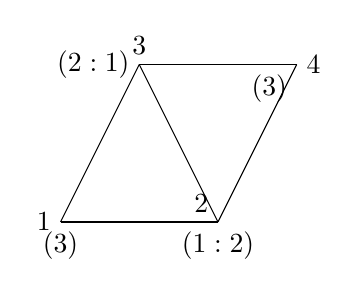
\begin{tikzpicture}
  \coordinate[label = left:$1$] (1) at (0,0);
  \coordinate[label = 135:$2$] (2) at (2,0);
  \coordinate[label = above:$3$] (3) at (1,2);
  \coordinate[label = right:$4$] (4) at (3,2);

  \coordinate[label = -90:$(3)$] (1loc) at (0,0);
  \coordinate[label = -90:$(1: 2)$] (2loc) at (2,0);
  \coordinate[label = left:$(2: 1)$] (3loc) at (1,2);
  \coordinate[label = -135:$(3)$] (4loc) at (3,2);

  \draw (1) -- (2);
  \draw (3) -- (2);
  \draw (1) -- (3);
  \draw (3) -- (4);
  \draw (2) -- (4);
\end{tikzpicture}

Es gibt zwei Möglichkeiten:
\begin{enumerate}
\item allgemeine Gültigkeit: Die Kantenbasisfunktioen werden im Referenzelement in beide Orienterungen definiert und die richtige auf Grundlage von \Lcode{orient} ausgewählt. (die 'falsche' ist der Teil der Papierkorbfunktion, DoF 0).
\item bei Punktsymmetrie ($Q_p$/ $P_p$-Elementen): Bei fehlender Orientierung reicht es, das Vorzeichen zu wechseln. Das Vorzeichen von \Lcode{orient} überträgt sich auf DoF und gibt an, dass der Negative der zugehörigen Referenzbasisfunktion durch $\Phi_K$ abgebildet wird. 
  \begin{align*}
    \phi_{ \norm{dA(i, k)}} (\hat \phi_i \circ \Phi_K^{-1}) \cdot \sign(cA(i, K))
  \end{align*}
\end{enumerate}
\begin{beispiel}
  zu (i): Betrachte die Skizze oben zu maximal kubischen Elementen. 
Basisfunktionen:
\begin{itemize}
\item $\phi_i$ linear, $i = 1, 2, 3$
\item $\phi_i$ quadratisch, $i = 4, 5, 6$
\item $\phi_i$ kubisch, $i = 7, \dots, 12$
\item $\phi_{13}$ im Inneren kubisch
\end{itemize}

  \begin{tabular}{c c}
    Kante Basisfunktion
$[1, 2]$& 5,6\\
$[1, 3]$& 1,3,4 \\
$[3, 4]$& 11,12\\
$[2, 4]$&9,10\\
$[2, 3]$&7,8\\
$Dreiec$k & Basisfunktion \\
$T_1$ & 15\\
$T_2$ & 16
  \end{tabular}

DoF-Manager:
\begin{align*}
  \begin{pmatrix}
    2 & 3\\
    3 & 2\\
    1 & 4\\
    7 & 7\\
    13 & 9\\
    5 & 11\
    8 & 0\\
    0 & 10\\
    6 & 0\\
    0 & 8\\
    13& 0\\
    0 &12 \\
    15&16
  \end{pmatrix}
\end{align*}

zu (ii): Basisfunktionen:
\begin{itemize}
\item $\phi_i$ linear, $i = 1, 2, 3$
\item $\phi_i$ quadratisch auf Kanten, $i = 4, 5, 6$
\item $\phi_i$ kubisch auf Kanten , $i = 7, \dots, 9$
\item $\phi_{10}$ im Inneren kubisch
\end{itemize}


DoF-Manager:
\begin{align*}
  \begin{pmatrix}
    2 & 3\\
    3 & 2\\
    1 & 4\\
    7 & 7\\
    13 & 9\\
    5 & 11\
    8 & -8\\
    -13 & 10\\
    5 & -12\\
    15&16
  \end{pmatrix}
\end{align*}
\end{beispiel}
\subsubsection{Vektorwärtige Finite-Element-Räume}
$V \leftrightarrow V_h$
\begin{align*}
  \cV = V \times V = V^2\\
\cV_h = V_h \times V_h = V_h^2
\end{align*}
mit $V_h = \Span \cB$ und $V_h^2 = (\Span \cB)^2 = \Span(\cB \otimes\cB)$ . 

\paragraph{Variante 1}: per Definition von vektorwärtigen Basisfunktionen. Sei  $  u_h \in V_h^2 $:
\begin{align*}
u_h = \sum_{i = 1}^{2N} c_i \vec \phi_i
\end{align*}
mit der Dimension $N$ von $V_h$
Vorteil: allgemein, insbesondere für nichttriviale vektorwärtige Elemente für $H(div)$, $H(rot)$ konforme Elemente
Nachteil: Mehr Aufwand

\paragraph{Variante 2}:
\begin{align*}
  V_h^2 = \Span \set{\cB \times \set 0, \set 0 \times \cB}
\end{align*}
$\vec \phi \in V_h^2$, 
\begin{align*}
  \vec \phi =
  \begin{pmatrix}
    \phi \\0 
  \end{pmatrix}
 \text{ oder }
  \begin{pmatrix}
    0\\\phi
  \end{pmatrix}, \qquad \phi \in V_h
\end{align*}
Vorteil: elegant, Nachteil: Funktioniert für diesen bestimmten Fall der Basiswahl
\begin{align*}
&  u_h = \sum_{i = 1}^{N} \vec c_i \phi_i\\
& \sum_{i = 1}^{2N} c_i \hat \phi_i =  \sum_{i = 1, 2, 2N-1} c_i
\begin{pmatrix}
  \phi(\frac i 2)\\0
\end{pmatrix}
+ \sum_{i = 2, 2, 2N} c_i
\begin{pmatrix}
0\\  \phi(\frac i 2)
\end{pmatrix}\\
&= \sum_{j = 1}^N c_{2j-1}
\begin{pmatrix}
  \phi_j \\0
\end{pmatrix} + \sum_{j = 1}^N c_{2j}
\begin{pmatrix}
  0\\\phi_j
\end{pmatrix}\\
&= \sum \underbrace{
\begin{pmatrix}
  c_{2j-1}\\c_{2j} 
\end{pmatrix}}_{\vec c_j}
\phi_j
\end{align*}
Damit lassen sich beliebige bereits implementierte DoF-Manager auf den vektorwäritgen Fall verallgemeinern. Jeder Eintrag in der DoFMap an Stelle $(i, K)$ repräsentiert zwei Freiheitsgrade $2i - 1$ und $2i$ (siehe in der Übung Lineare Elastititätstheorie und Stokes-Problem)
\begin{beispiel}
Betrachte

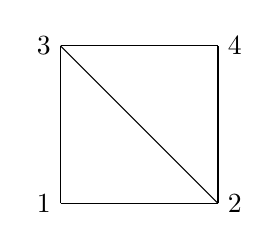
\begin{tikzpicture}
  \coordinate[label = left:$1$] (1) at (0,0);
  \coordinate[label = right:$2$] (2) at (2,0);
  \coordinate[label = left:$3$] (3) at (0,2);
  \coordinate[label = right:$4$] (4) at (2,2);

  \draw (1) -- (2);
  \draw (3) -- (2);
  \draw (1) -- (3);
  \draw (3) -- (4);
  \draw (2) -- (4);
\end{tikzpicture}  

mit lokaler Nummerierung

\begin{tabular}{c c}
  $T_1$&$2 -3-1$\\
  $T_2$&$3 -2-4$
\end{tabular}.

Skalarer Fall:
\begin{align*}
  dM =
  \begin{pmatrix}
    2 & 3 \\
    3 & 2\\
    1 & 4
  \end{pmatrix}
\end{align*}
Freiheitsgrade: 
\begin{align*}
&  1 = 2 \cdot 1 - 1 \leftrightarrow \phi_1 =
  \begin{cases}
    \begin{pmatrix}
      1-x-y\\ 0
    \end{pmatrix} & T_1\\
    \begin{pmatrix}
      0\\ 0
    \end{pmatrix} & T_2\\
  \end{cases}\\
 & 2 = 2 \cdot 1 - 0 \leftrightarrow \phi_2 =
  \begin{cases}
    \begin{pmatrix}
      0\\1-x-y
    \end{pmatrix} & T_1\\
    \begin{pmatrix}
      0\\ 0
    \end{pmatrix} & T_2\\
  \end{cases}\\
 & 3 = 2 \cdot 2 - 1 \leftrightarrow \phi_3 =
  \begin{cases}
    \begin{pmatrix}
      x\\ 0
    \end{pmatrix} & T_1\\
    \begin{pmatrix}
      1-y\\ 0
    \end{pmatrix} & T_2\\
  \end{cases}\\
&  4 = 2 \cdot 2 - 0 \leftrightarrow \phi_1 =
  \begin{cases}
    \begin{pmatrix}
      0\\x
    \end{pmatrix} & T_1\\
    \begin{pmatrix}
      0\\ 1-y
    \end{pmatrix} & T_2\\
  \end{cases}
\end{align*}

\end{beispiel}
\subsection{Der Finite Elemente Raum \Lcode{FESpace} }

\begin{itemize}
\item Durch 
\framebox{Mesh$\stackrel{\text{DoF-Manager}}{\longleftrightarrow}$Element}$_{\text{FESpace}}$
 ist der FE-Raum $V_h$ vollständig beschrieben.
\item \Lcode{FESpace} ist/erbt von \Lcode{MeshObserver} und hat \Lcode{Mesh} als Membervariable
\item zusätzliche Membervariablen von FE-Space: mesh, element, quadRule, DoFManager
\item Hauptaufgabe: Modifikation und Auswertung von DoFVektoren, Assemblierung von Operatoren/Projektoren auf $V_h$ beziehungsweise nach $V_h$
\end{itemize}
Konkret lauten die Aufgaben:
\begin{itemize}
\item Auswertung von FE-Funktionen (punktweise)
(Vektor von Freiheitsgraden $\R^{nDoF \times 1}$ $\leftrightarrow$ Funktionswärtig in lokalen Punkten $\R^{nE \times nP}$)
\item Abfrage von Daten in den Quadraturpunkten (Koeffizienten, Referenzabbildung, ,$(\det(D \Phi_K))_K$, Normalenvektor)
\item Assemblierung grundlegender Operatoren, Funktionale (zum Beispiel Massematrix, $(\int f \phi_i)_{i = 1}^{nDoF}$)
\item Interpolation von beliebigen Funktionen in FE-Raum
\item Projektionen zwischen zwischen verschiedenen Gitterlevels/ bzw um hängende Knoten zu behandeln. 
\item Modifikationen von DoFVektoren:
\begin{align*}
&  f(u_h) = v_h\\
& \nabla u_h \\
& \int u_h
\end{align*}
\item Visualisierung von FE-Funktionen
\item get- und set-Funktionen
\end{itemize}

%\datum{18. Dezember 2014}
\subsubsection{Auswertung von FE-Funktionen (DoF-Vektoren)}
Sei $V_{h}$ Finite Elemente Raum, $v_{h} \in V_{h}$ Finite Elemente Raum. 
\begin{uebung*}
  Gegeben sei $v_{h} \in \R^{nDoF}$, $\set{\hat x_{i}}_{i = 1}^{nP} \subset \hat K$, 

Gescuht ist $\set{v_{h} (\Phi_{k(\hat x_{i})})}_{i = 1, \dots, nD, k = 1, \dots, nE} $, $V_{h} : \Omega_{h} \to \R$ ($v_{h} \tilde = \R^{nDoF})$
\begin{align*}
  v_{h}(\phi_{k(\hat x_{i})}) &= \sum_{J = 1}^{nDoF} v_{J}\phi_{J}(\Phi_{k}(x_{i}))\\
&= \sum_{j = 1}^{nDoF} v_{dM(j, k)} \underbrace{\phi_{j}\circ\Phi_{k}}_{{\hat \phi_{j}}}(x_{i})\\
&= \set{\sum_{j = 1}^{nDoF} v_{dM(j, k)}\hat \phi_{j}(\hat x_{i})}_{i = 1, \dots nP, j = 1, \dots, nE}\\
\end{align*}
(Beiträge nur für $\supp \phi_{J} \cap K_{k} \neq \emptyset$)

Hierbei entsprechen die $\hat x_{j}$ \Lcode{points} und $\hat \phi_{j}(\hat x_{i})$ \Lcode{basis = element.getbasis(points, 0)}

\Lcode{

recall DoFMap valuesAtDoF
  \begin{align*}
&    \begin{pmatrix}
      1 & 3\\ 5 & 6 \\ \vdots & \vdots \\ -81 & 0 \\ \vdots & \vdots
    \end{pmatrix} 
\Rightarrow 
    \begin{pmatrix}
      v_{11} & v_{12}\\ &\\ \vdots & \vdots \\ & \\ \vdots & \vdots
    \end{pmatrix} 
\\
&nB \times nE \Rightarrow \dots
  \end{align*}
doFMap = obj.getDoFMap

i = doFMap $\neq 0$

valuesAtDoFs = zeros(size(doFMap))

valuesAtDoFs(I) = sign(doFMap(I)).* $V_n$(abs(doFMap(I))) $\in \R(nB, nE)$

R = valuesAtDoF's *basis}

\Lcode{ 
basis = permute(basis $[3, 2, 1]$) $\in \R(1, nP, nB)$

value = permute(value $[2, 3, 1]$) $\in \R(ne, 1, nB)$

R =  sum(bsxfun(@times, basis, value), 3)} (schöner / langsamer?!)
\Lcode{bsxfun(@times, basis, value) $\in \R(nE, nP, nB)$}
\end{uebung*}
\paragraph{Lokale Auswertung für $\nabla$}
\begin{align*}
  \set{\nabla v_{h}( \Phi_{k}( \hat x_{i}))}_{k, i} = \set{\sum_{j = 1}^{nB} v_{dM(j, k)} \nabla \phi_{dM(j, k)}(\Phi_{k}(\hat x_{i}))}
\end{align*}
Nebenrechnung:
\begin{align*}
&\nabla \phi \circ \nabla (\phi \circ \Phi)  \\
&D(\phi \circ \Phi) = D\phi \circ \Phi \cdot D\Phi\\
&\nabla(\underbrace{\phi \circ \Phi}_{\hat \phi}) = D\phi^{T} (\nabla \phi \circ \Phi)\\
&\nabla\phi \circ \Phi = D\phi^{-1 \circ T} \nabla \hat \phi)\\
&= \set{\sum_{j} v_{dM(j, k)} D \Phi^{-T} \nabla \hat \phi(\hat x_{i})}_{k, i} = R
\end{align*}
\subsubsection{Quadratur}
Typische Integrale (s. Assemblierung) haben die Form 
\begin{align*}
  I = \int_{\hat K} \underbrace{c \delta_{s}^{i} \hat \phi \delta_{t}^{j} \hat\psi \norm{\det D \Phi_{k}}}_{\Lambda(\hat x)} d \hat x, i, j = 0, 1, \dots, s, t \in \set{\hat x, \hat y}
\end{align*}
\begin{itemize}
\item mögliche Auswertungen: symbolisch oder numerisch
\item $I$ kann exakt berechnet werden, falls $\Phi_{k}$ linear und $C$ konstant ist 
\item Die exakte Auswertung ist nicht nötig, um eine optimale Konvergenzordnung zu erreichen, da die Diskretisierung sowieso Fehler liefert. 
\item Ziel: möglichst hohe Genauigkeit bei minimaler Anzahl von Funktionsauswertungen
  \begin{align*}
    I \approx \sum_{k = 1}^{nQ}\omega_{k} \Lambda(\hat x_{k})
  \end{align*}
(Gaußquadratur)
\end{itemize}
\paragraph{Gauß-Quadratur}
\begin{itemize}
\item Typischerweise auf (-1, 1)
  \begin{align*}
    \set{\hat x_{k}, \omega_{k}}_{k} \text{ so, dass } \sum_{k = 1}^{nQ} \omega_{k} p(\hat x) d \hat x \qquad \forall p \in \Pi_{N}, N >> 1
  \end{align*}
Daraus folgt ein nichtlineares Gleichungssystem für $2 nQ$ Unbekannte der Dimension $\Pi_{N} = N+1$. Also $N = 2nQ-1$ 
\end{itemize}
\begin{beispiel}
  \begin{align*}
    \int_{-1}^{1} g(\hat x) d \hat x \approx \frac {1}{g}(5g(- \sqrt{\frac 3 5}) + 8g(0) + 5g(- \sqrt{\frac 3 5}))
  \end{align*}
\end{beispiel}
Theorie: $\set {\hat x_{k}}$ sind die Nullstellen der Legendre-Polynome

\paragraph{2D-Vierecke} auf $(-1, 1)^{2}$: 

Einfacher Tensoransatz: $M= nQ$

\begin{align*}
  \set{\hat x_{k}^{2D}}_{k= 1}^{M^{2}} = \set{\hat x_{k}^{1D}} \times\set{\hat x_{k}^{1D}}_{k = 1}^{m}\\
(\omega_{k_{k}}^{2D})_{k} = (\omega_{k}^{1D}) \otimes (\omega_{k}^{1D})
\end{align*}

\paragraph{2D-Dreiecke}
\begin{enumerate}
\item Variante 1: Gegeben $(\hat x_{k}, \omega_{k})_{k}$ auf $(0, 1)^{2}$

Abbildung des Vierecks auf ein Einheitsdreieck durch $T$ entlang von Isolinien.
\begin{align*}
&  p = T(q) =
  \begin{pmatrix}
    q_{1}(1-q_{2})\\ q_{2}
  \end{pmatrix}
\\
& \int_{p \in \Delta} f(p) dp = \int_{q \in T^{-1}(\Delta)} f(T(q))\norm{J_{T}} dq \\
= \int_{\square} (1-q_{2})f(T(q)) dq
&\approx \underbrace{\sum w_{k}(1- \hat x_{k, 2})}_{\omega_{k}^{\Delta}}\underbrace{f(T(\hat x_{k}))}_{\hat x_{k}^{\Delta}}
\end{align*}
Nachteil: leichter Overhead, nicht symmetrisch

Vorteil: nicht Nachteil (ii)
\item Variante 2: Optimale Gaußquadratur
  \begin{itemize}
  \item Aufstellen von nichlinearem Gleichungssystem bezüglich optimaler Punkte und Gewichte mit Ziel
    \begin{align*}
      \int_{\Delta} g(\underbar x) d\underbar x
    \end{align*}
%exakt für $g \in \Span \set{x^{i}y^{i}|\; 0 \leq i, j, i+j \leq N} = P_{N}$, $N$ groß. Daraus entstehe ein nichtlineares Gleichungssystem für $3 nQP$, $\dim P_{N} = \frac {(N+1)(N+2)2}$
\begin{align*}
  nQP^{\Delta} = \ceil{\frac {(N+1)(N+2)}6}
\end{align*}
versus
\begin{align*}
  nQP^{\square} = \ceil{\frac {N+1}2}^{2}
\end{align*}
  \end{itemize}
Nachteil:
\begin{itemize}
\item aufwändig zu berechnen
\item geht nur tabelliert im Code ein
\item Gegenstanda aktueller Forschung
\end{itemize}
Vorteil: nicht  (Nachteil oben)
\end{enumerate}

\begin{tabular}{c| c |c}
N &$\triangle$  & $\square$ \\\hline
1 & 1& 1\\
2 & 2& 4\\
3 & 4& 4\\
4 & 5& 9\\
5 & 7& 9\\
6 & 9& 16\\
7 & 12& 16
\end{tabular}

QuadRule hat eine abstrakte Methode \Lcode{getData()}, welche beim Erstellen des konkreten Quadratur-Objektes aufgerufen wird unf QP, Qgew in properties speichert. FESpace stellt Methoden zur Verfügung, welche in QP liefert...

\begin{tabular}{c|c|c}
  Daten & DoFVectors & Referenzabbildung\\ \hline
\Lcode{evalFunctionIQP()}&\Lcode{evalDoFVectorIQP} & \Lcode{evalDef-MapQP}\\
&&\Lcode{evalTrafoIQP()}\\
&&\Lcode{(evalNormalVectorIQP)}\\
\end{tabular}

%\datum{06. Januar 2015}

Prüfung: kleine Projekte + mündlicher Anteil 

\subsubsection{Assemblierung}

\begin{align*}
&  - \Delta u + b \cdot \nabla u + cu = f
&a(u, v) = f(v)\qquad \forall v \in V = H_{0}^{1}(\Omega)
\end{align*}
\begin{align*}
&  <\cL u , v>_{V' \times V} = \int \nabla u \cdot \nabla v d u + \int b \cdot \nabla u v dx + \int c u v \, dx = \int f v \, dx = <f, v>_{V' \times V}\\
&\cL: V \to V'\\
&\cL_{h}: V_{h} \to V_{h}' \in R^{nDoF \times nDoF}\\
&f \in V'\\
&f_{h} \in V'_{h} \in \R^{nDoF}?
\end{align*}
\enu{\roman}
\begin{enumerate}
\item $L_2$-Skalarprodukt
  \begin{align*}
    f_{h} &= \set{\int_{\Omega_{h}} f v_{h} dx}_{v_{h} \in V_{h}} |_{\bar \O_{h} = \bigcup \cT_{h}}\\
&= \set{\sum_{K \in \cT_{h}}\int_{K} f v_{h} dx}_{v_{h} \in V_{h}} \text{ (teste nur mit $\phi_{I} \in \cB_{V_{h}}$)}\\
&= \set{\sum_{K \in \cT_{h}}\int_{K} f v_{I} dx}_{I = 1, \dots, nDoF} 
  \end{align*}
Es reicht diejenigen $\phi_{I}$'s auf $K$ zu betrachten, welche $\supp \phi_{I} \cap K \neq \emptyset$ $(*)$ erfüllen, das führt zur Betrachtung lokaler Basisfunktionen. 

Transformation: 
\begin{align*}
&  \Phi_{K}: \hat K \to K\\
&dx = \norm{D \Phi_{K}} d \hat x\\
&x = \Phi(\hat x)\\
\Rightarrow &= \set{\sum_{K: (*)} \int_{\hat K} \left(\underbrace{f \circ \Phi_{K}}_{\hat f}\right)\left( \phi_{I} \circ \Phi_{K} \right)\norm{D \Phi_{K}} d \hat x}_{I}\\
 &= \stackrel{dMap}{\Big{\alpha}}\set{\int_{\hat K} \hat f \hat \phi_{i} \norm{D \Phi_{K}} d \hat x}_{i = 1 \dots, nB, k = 1, \dots, nE}\\
 & \approx \stackrel{dMap}{\Big{\alpha}}\set{\sum_{q = 1}^{nQ} \hat f(\hat x_{q}) \cdot \hat \phi_{i}(\hat x_{q}) \norm{D \Phi_{K}(\hat x_{q})} w_{q}}_{i = 1 \dots, nB, k = 1, \dots, nE}
\end{align*}
$\alpha$: Schreibe an die Richtige Stelle und summiere auf (Assemblierung).

Zutaten: 
\begin{itemize}
\item \Lcode{weights} $w \in \R(nQ, 1)$\Lcode{obj.getQuadData(d1)} (Codimension)
\item \Lcode{points} $\hat x \in \R(nQ, nD)$\Lcode{obj.getQuadData(d1)} (Codimension)
\item \Lcode{F} $F \in \R(nE, nQ)$ \Lcode{obj.mesh.evalFunction(f_h, points)}
\item \Lcode{basis} $\set{\phi_{i(\hat x _{q})}} \in \R(nB, nQ)$ \Lcode{obj.element.getBasis(points, 0)}
\item \Lcode{trafo} $\set{\norm{D \Phi_{k}(\hat x_{q})}_{q}}\in \R(nE, nQ)$ \Lcode{obj.mesh.getTrafo(points)}
\end{itemize}

Schritte
\begin{itemize}
\item \Lcode{entry = bsxfun(@times, $\overbrace{\text{F.*trafo}}^{\R(nE, nQ)}$, weights')* $\underbrace{\text{basis'}}_{\R(nQ \times nB)}$ }$\in \R(nE, nB)$
\item \Lcode{[dMap, nDoF] = obj.getDoFMap(codim)} $\in \Z(nE, nB)$
\item \Lcode{entry(dMap $<$ 0) = -entry(dMap)}
\item \Lcode{I = (dMap $\neq$ 0)}
\item \Lcode{F = full(sparse(abs(dMap(I)), ones(size(dMap(I)), entry(I)m nDoF, 1)))}
\end{itemize}

\item Massematrix
  \begin{align*}
    <\cLu, v> = \int_{\O} c u v \, dx  \\
    <\cL_{h}u_{h}, v_{h}> = \int_{\O_{h}} c u_{h} v_{h} \, dx  \\
\cL_{h} u_{h} = \set{\sum_{K} \int_{K} c u_{h} v_{h} dx}_{v_{h} \in V_{h}}\\
= \set{\sum_{K} \int_{K} c \left(\sum_{j} u_{j}  \phi_{j}\right) \phi_{I} dx}_{I = 1, \dots, nDoF}}\\
= \underbrace{\set{\sum_{K: (*)} \int_{K} c  \phi_{J} \phi_{I} dx}_{I = 1, \dots, nDoF}}}_{\cL_{h}} \cdot \set{\phi_{J}}_{J = 1, \dots, nDoF}\\
 = \stackrel{dMap}{\Big{\alpha}}\set{\int_{\hat K}  c \circ \Phi_{K} \hat \phi_{j}  \hat \phi_{i} \norm{D \Phi_{k}} d \hat x}_{i, j = 1, \dots, nB, k = 1, \dots, nE}\\
 = \stackrel{dMap}{\Big{\alpha}}\set{\sum_{q}}  \hat c(\hat x_{q}) \hat \phi_{j}(\hat x _{q}) \hat \phi_{i} (\hat x _{q}) T_{k}(\hat x _{q}) w_{q}}_{i, j = 1, \dots, nB, k = 1, \dots, nE}\\
  \end{align*}
mit $\norm{D\Phi_{k}} = T_{k}$ und $\hat c = c \circ \Phi_{k}$ und $(*) : \supp \phi_{J} \cap \supp \phi_{I} \cap K \neq \emptyset$ und den Zutaten
\begin{itemize}
\item \Lcode{weights, points, c, basis, trafo} wie in (i)
\end{itemize}
Schritte: 
\begin{itemize}
\item \Lcode{basisI = reshape(basis, 1, nB, nQ)}
\item \Lcode{basisJ = reshape(basis, nB, 1, nQ)}
\item \Lcode{basisIbasisJ = bsxfun(@times, basisI, basisJ)} $\in \R(nB, nB, nQ)$ (i, j, q)
\item \Lcode{data = bsxfun(@times, C.*trafo, weights)} $\in \R(nE, nQ)$
\item \Lcode{entry = reshape(basisIbasisJ, nB$^{2}$, nQ)*data'} $\in \R(nB^{2}, nE)$
\item \Lcode{[dMap, nDoF] = obj.getDoFMap(codim)} $\in \R(nB, nE)$
\item \Lcode{dMapI = kron(ones(nB, 1), dMap)}
\item \Lcode{dMapJ = kron(dMap, ones(nB, 1))}
\item \Lcode{entry(dMapI*dMap $<$ 0) = -entry(\dots)}
\item \Lcode{I = dMapI $\neq$ 0 und dMapJ $\neq$ 0}
\item \Lcode{M = sparse(abs(dMapI(I), abs(dMapJ(I)), entry(I), nDoF, nDoF)}
\end{itemize}
Kroneckerprodukt von Matrizen: Jedes Element der ersten Matrix wird mit der zweiten Matrix multipliziert.  

%\datum{08. Januar 2014}

\item Schwacher Laplace-Operator 
  \begin{align*}
    \int_{\Omega} a \nabla u \cdot \nabla v dx &= <\cLu, v>_{V \times V'}\\
    <\cL_{h}u_{h}, v_{h}> &=  \int_{\Omega_{h}} a \nabla u_{h} \cdot \nabla v_{h} dx\\
    \cL_{h}u_{h} &=  \set{\sum_{K}\int_{K} a \nabla u_{h} \cdot \nabla v_{h} dx}_{V_{h}}\\
    &=  \set{\sum_{K}\sum_{J} u_{J} \int_{K}a \nabla \phi_{J} \cdot \nabla \phi_{I} dx}_{I = 1, \dots, cDoF}\\
    &=  \underbrace{\set{\sum_{K}int_{K}a \nabla \phi_{J} \cdot \nabla \phi_{I} dx}_{I = 1, \dots, cDoF}}_{\cL_{h}} * \set{u_{J}}_{J}\\
    \cL_{h}u_{h} &= \set{\sum_{K: (*)} \int_{K} a \nabla \phi_{J} \cdot \nabla \phi_{I} dx}_{I, J}\\
    &= \set{\sum_{K: (*)} \int_{K} a \nabla \phi_{J} \cdot \nabla \phi_{I} dx}_{I, J}\\
 &= \stackrel{dM}{\Big{\alpha}} \set{\int_{\hat K} \underbrace{a \circ \Phi_{k}}_{\hat a _{k}} \left( \left(\nabla \phi_{dM(j, k)}\right) \circ \Phi_{k}\right) \left(\left( \nabla\phi_{dM(i, k)}\right) \circ \Phi_{k}\right) \norm{D\Phi_{k}} d \hat x}_{i, j = 1, \dots, nB, k = 1, \dots, nE}\\
 &= \stackrel{dM}{\Big{\alpha}} \set{\int_{K} \hat a _{k} \left( D\Phi_{k}^{-T}\nabla\hat \phi_{j}\right) \left(D\Phi_{k}^{-T}\nabla\hat\phi_{i}\right) \norm{D\Phi_{k}} d \hat x}\\
 &= \stackrel{dM}{\Big{\alpha}} \set{\sum_{q} \hat a _{k_{q}} \underbrace{\underbrace{\left( D\Phi_{k}^{-T}\nabla\hat \phi_{j}\right)_{q}}_{dBasisG_{jqk}} \left(D\Phi_{k}^{-T}\nabla\phi_{i}\right)_{q}}_{[\cdot]_{x}[\cdot]_{x} + [\cdot]_{y}[\cdot]_{y}} \norm{D\Phi_{k}}_{q} W_{q}}
\end{align*}
mit Bedingung $(*):\; \supp \phi_{J} \cap \supp \phi_{I} \cap K \neq \emptyset$ und $x = \Phi_{K}(\hat x)$.

Zutaten: 
\begin{itemize}
\item \Lcode{weights} $\in \R(nQ, 1)$
\item \Lcode{points} $\in \R(nQ, nD)$, $nD = 2$
\item \Lcode{A} $\in \R(nE, nQ)$
\item \Lcode{dBasisG} $\in \R(nD, nB, nE, nQ)$, siehe nächster Abschnitt
\item \Lcode{trafo} $\in \R(nE, nQ)$
\end{itemize}
Schritte:
\begin{itemize}
\item Felder: \Lcode{doFMapI, doFMapJ} siehe Massematrix
\item Feld für Einträge \Lcode{entry}
\item dann $\cL_{h}= $\Lcode{sparse(doFMapI, doFMapJ, entry)}
\end{itemize}
\Lcode{entry = bsxfun(@times, A.*trafo, weights')} $\in \R(nE, nQ)$

\Lcode{dxBasisGI = reshape(dBasisG(1, :), 1, nB, nE, nQ)}

\Lcode{dxBasisGJ = reshape(dBasisG(1, :), nB, 1, nE, nQ)}

\Lcode{dxdx = bsxfun(@times, dxBasisI, dyBasisJ)} $\in \R(nB, nB, nE, nQ)$

\Lcode{dyBasisGI = reshape(dBasisG(2, :), 1, nB, nE, nQ)}

\Lcode{dyBasisGJ = reshape(dBasisG(2, :), nB, 1, nE, nQ)}

\Lcode{dydy = bsxfun(@times, dxBasisI, dyBasisJ)} $\in \R(nB, nB, nE, nQ)$

\Lcode{entry = bsxfun(@times,  reshape(entry, 1, 1, nE, nQ), dxx, dyy)}

\Lcode{entry = sum(entry, 4)}
\Lcode{entry = reshape(entry, nB$^{2}$), E} (Rest wie in (ii))

\begin{bemerkung}
  Nach Berechnung von \Lcode{dBasisG} lässt sich die Assemblierung in einer!! Zeile schreiben :)
\end{bemerkung}
\item Transformation von Ableitungen (erste und zweite)

Bekannt: 
\begin{align}
  x &= \Phi(\hat x) \label{eq:arg}\\
\phi(x) &= \hat \phi (\hat x) \label{eq:D0}\\
\nabla \phi(x) &= D\Phi^{-T}(\hat x)\nabla\hat \Phi(\hat x) \label{eq:D1}
\end{align}
Die zweiten Ableitungen werden auch gebraucht, zum Beispiel bei Stomliniendiffusion, residualen Fehlerschätzern. 
\begin{align}
  D\nabla\phi\left(x\right) \cdot D \Phi\left(\hat x\right)&= \underbrace{D\left(D\Phi^{-T}\left(\hat x\right)\right) \nabla \hat\phi\left(\hat x\right)}_{= 0 \text{ auf gradlinig berandeten El.}} + D\Phi^{-T}\left(\hat x\right) D \nabla \hat \phi \left(\hat x\right) \notag\\
\nabla^{2}\phi(x) &= D\Phi^{-T}\nabla^{2}\hat\phi(\hat x) D \Phi^{-1} \label{eq:D2}
\end{align}
Umsetzung in Matlab (vektorisiert): 
\begin{itemize}
\item \eqref{eq:D0} \Lcode{getBasis(points, 0)}
\item \eqref{eq:D1} Matrix-Vektor-Multiplikation

\Lcode{trafoInv = obj.mesh.evalInvJacobian(points)} \in $\R(nD_{i}, nD_{j}, nE, nP)$ calls \Lcode{evalReferenceMap(points, 1)}

\Lcode{trafoInv = permute(trafoInv, [1 2 3 5 4])}

\Lcode{ dBasis = obj.element.getBasis(points, 1)} $\in \R(nB, nP, bD_{i})$ 

\Lcode{ dBasis = permute(dBasis, [3 4 5 1 2])}

\Lcode{R = sum(bsxfun(@times, trafoInv, dBasis), 1)}

\Lcode{R = permute(R, [3 4 5 2 1])}
\end{itemize}
\begin{bemerkung}
  Einzeiler :)
\end{bemerkung}
\end{enumerate}
\subsubsection{Interpolation in den FE-Raum}
Zur Erinnerung: $V$ ist ein Hilbertraum in variationeller Formulierung. $V_{h} \subset V$ ist ein endlichdimensionaler Finite-Elemente-Raum. 

Aufgabe: Für $g \in V$ finde $g_{h} \in V_{h}$ mit guten Approximationseigenschaften, das heißt $\nnorm{g - g_{h}}$ wird klein. Finde eine Abbildung $I: \; V \to V^{h}$ mit $\nnorm{g - Ig}$ klein.

Klassisches Vorgehen: Vermesse $g$ und $V^{h}$ mittels einer linearen, stetigen Funktion. Seien $f_{i} \in V' = \cL_{b}(V, \R), \, i = 1, \dots, M$. Eigenschaften von $I$:
\begin{align}{eq:I}
  f_{i}(Ig) = f_{i}(g), \quad i = 1, \dots, M.
\end{align}
Außerdem
\begin{align*}
  g^{h}\coloneqq Ig \lognrightarrow Ig = \sum_{j = 1}^{N}g_{j}\phi_{j} 
\end{align*}
($N = nDoF$). Mit \eqref{eq:I} folgt
\begin{align*}
  \sum_{j=1}^{N} \sunderbrace{g_{j}f_{i}(\phi_{j})}_{{A_{ij}}} = \underbrace{f_{i}(g)}_{F_{i}}, \quad i = 1, \dots, M
\end{align*}
führt auf das lineare Gleichungssystem 
\begin{align}\label{eq:lgs}
  A g = F.
\end{align}
Wir nennen $(V_{h}, \set{f_{i})_{i = 1}^{N}}$ unisolvent, wenn $Ag = F$ eine eindeutige Lösung hat. Da $M = N$ sein soll und $(f_{i}(\phi_{j}))_{ij}$ muss regulär sein. DAmit beschreibt \eqref{eq:I} eine eindeutige Abbildung. Konkrete Wahl von $\set{f_{i}}_{i = 1}^{nDoF}$ beschreibt konkrete Interpolation. 
\begin{beispiel}
Mittels \eqref{eq:I} und \eqref{eq:lgs}:
  \begin{align*}
&    f_{i} = g \mapsto \int_{\O}g f_{i}dx = (g, \phi_{i})_{L_{2}}, \quadi = 1, \dots, nDoF\\
\Rightarrow & (Ig, \phi_{i}) = (g_{i, \phi_{i}})\\
&(Ig - g, \phi_{i}) = 0 \quad L_{2}\text{-Projektion}
\Rightarrow& Ag = F \text{ mit } A = ((\phi_{j}, \phi_{i}))_{ij}, F = ((g, \phi_{i}))_{i = 1}^{\nDoF}
\end{align*}
Regularität von $A$:

Betrachte $v \in \R^{N}\setminus\set{0}$ (entspricht  $v_{h} = \sum v_{i} \phi_{i}$)
\begin{align*}
  v^{T}Av = \sum_{ij} v_{i}v_{j}(\phi_{j}, \phi_{i}) = (v_{h}, v_{h}) = \nnorm{v_{h}}^{2} > 0
\end{align*}
Daher ist $A$ positiv definit und somit regulär ($v_{i} \neq 0$, da $v \neq 0$ und $\phi_{i}$ linear unabhängig)
\end{beispiel}
Im Code:

\Lcode{
U = evalGlobalL2Projection(obj, f)

M = obj.assembleMassMatrix(@(x)x(:, 1).10, 0)

F = obj.assembleL2Product(f,0)

U = M\F;}
\begin{beispiel}
  \begin{align*}
    b_{i} = g \mapsto a(G, \phi_{I}), \quad i = 1, \dots, nDoF
  \end{align*}
definieren die sogenannte Ritz-Projektion. 
Regularität von $(a(\phi_{j}, \phi_{i}))_{ij}$ filgt aus der Koerzivität von $a(\cdot, \cdot)$ über $V_{h}$. (Wie im ersten Beispiel)
\end{beispiel}
\begin{beispiel}
  In dein vorangegangenen Beispielen ist $f_{i}$ ein globaler Interpolator, das heißt, das Lösen eines globalen linearen Gleichungssystems ist notwendig :(. Besonders einfach: Lagrange-Interpolation.
  \begin{align*}
    f_{i} &= \delta_{x_{i}}\\
f_{i}(g) &= g(x_{i})\\
f_{i}(\phi_{j}) &= \phi_{j}(x_{i}) = \delta_{ij} = I d_{\R^{N \times N}} = A
  \end{align*}
\end{beispiel}
\begin{beispiel}
  Lokale $L_{2}$-Projektion: O.E.d.A. sei $p$ der Polynomgrad auf allen Elementen. 
  \begin{align*}
&    nDoF = nN + nF(p-1) + nE, \quad\text{nN = #Knoten, nF = #Kanten, nE = #Elemente}\\
& f_{i}^{N} g = g(x_{i}), \quad i = 1, \dots, nN\\
& V^h = V^h_{N} \setproduct V^h_{F} \setproduct V^h_{E}
  \end{align*}
$f_{i}^{N}$: Definierter Interpolator von $V \to V_{N}^{h}$. 
\begin{align*}
&  f_{j}^{F}g = \int_{F} g \phi_{dM^{F}(j+2), F} ds, \quad j = 1, \dots, p-1\\ 
&  f_{j}^{E}g = \int_{E} g \phi_{dM^{E}(j+p\cdotnV), E} ds
\end{align*}
\end{beispiel}
\begin{beispiel}
  Randprojektion
  \begin{align*}
    &I_{\partial \Omega}: L_{2}(\partial \Omega) \to V^{h}|_{\partial \Omega}\\
    &i \in dM(:, F)
  \end{align*}
ist definiert durch zum Beispiel $f_{i} = g \mapsto \int g \phi_{i} ds$. Zur Approximation von Randdaten: siehe Operatorklasse, Dirichletrandbedingung. Billiger als die volle $L_{2}$-Projektion.
\begin{align*}
  &I : H^{\frac 1 2}(\O) \to V^{h}\\
  &I : P^{\O} I_{\partial \O}R^{\partial \O} g
\end{align*}
mit $P$: Prolongation durch $0$, $R^{\partial \O}: H^{\frac 1 2}(\Omega) \to L_{2}(\partial \O)$ (Spur-Operator) 
\end{beispiel}
Praktisch: im FESpace 

\Lcode{

U = obj.evalBoundaryProjection(f, [location])

I = obj.mesh.isBoundaryFace([location])

M = obj.assembleMassMatrix(@(x)1 + 0*x(:, 1), 1, I)

 assembleL2Projection(f, 1, I)

U = zeros(size(F))

dMap = obj.getDoFMap(1)

$\I$ = setdiff(unique(dMap(., I)), 0)

U($\I$) = M($\I$, $\I$)$\setminus$ F($\I$)
}

location: zum Beispiel $x + y > 1$ als Dirichlet-Randbedingung

